\documentclass[]{article}
\usepackage{lmodern}
\usepackage{amssymb,amsmath}
\usepackage{ifxetex,ifluatex}
\usepackage{fixltx2e} % provides \textsubscript
\ifnum 0\ifxetex 1\fi\ifluatex 1\fi=0 % if pdftex
  \usepackage[T1]{fontenc}
  \usepackage[utf8]{inputenc}
\else % if luatex or xelatex
  \ifxetex
    \usepackage{mathspec}
  \else
    \usepackage{fontspec}
  \fi
  \defaultfontfeatures{Ligatures=TeX,Scale=MatchLowercase}
\fi
% use upquote if available, for straight quotes in verbatim environments
\IfFileExists{upquote.sty}{\usepackage{upquote}}{}
% use microtype if available
\IfFileExists{microtype.sty}{%
\usepackage{microtype}
\UseMicrotypeSet[protrusion]{basicmath} % disable protrusion for tt fonts
}{}
\usepackage[margin=1in]{geometry}
\usepackage{hyperref}
\hypersetup{unicode=true,
            pdftitle={Monte Carlo Methods},
            pdfauthor={Edward Ionides},
            pdfborder={0 0 0},
            breaklinks=true}
\urlstyle{same}  % don't use monospace font for urls
\usepackage{graphicx,grffile}
\makeatletter
\def\maxwidth{\ifdim\Gin@nat@width>\linewidth\linewidth\else\Gin@nat@width\fi}
\def\maxheight{\ifdim\Gin@nat@height>\textheight\textheight\else\Gin@nat@height\fi}
\makeatother
% Scale images if necessary, so that they will not overflow the page
% margins by default, and it is still possible to overwrite the defaults
% using explicit options in \includegraphics[width, height, ...]{}
\setkeys{Gin}{width=\maxwidth,height=\maxheight,keepaspectratio}
\IfFileExists{parskip.sty}{%
\usepackage{parskip}
}{% else
\setlength{\parindent}{0pt}
\setlength{\parskip}{6pt plus 2pt minus 1pt}
}
\setlength{\emergencystretch}{3em}  % prevent overfull lines
\providecommand{\tightlist}{%
  \setlength{\itemsep}{0pt}\setlength{\parskip}{0pt}}
\setcounter{secnumdepth}{0}
% Redefines (sub)paragraphs to behave more like sections
\ifx\paragraph\undefined\else
\let\oldparagraph\paragraph
\renewcommand{\paragraph}[1]{\oldparagraph{#1}\mbox{}}
\fi
\ifx\subparagraph\undefined\else
\let\oldsubparagraph\subparagraph
\renewcommand{\subparagraph}[1]{\oldsubparagraph{#1}\mbox{}}
\fi

%%% Use protect on footnotes to avoid problems with footnotes in titles
\let\rmarkdownfootnote\footnote%
\def\footnote{\protect\rmarkdownfootnote}

%%% Change title format to be more compact
\usepackage{titling}

% Create subtitle command for use in maketitle
\newcommand{\subtitle}[1]{
  \posttitle{
    \begin{center}\large#1\end{center}
    }
}

\setlength{\droptitle}{-2em}
  \title{Monte Carlo Methods}
  \pretitle{\vspace{\droptitle}\centering\huge}
  \posttitle{\par}
  \author{Edward Ionides}
  \preauthor{\centering\large\emph}
  \postauthor{\par}
  \predate{\centering\large\emph}
  \postdate{\par}
  \date{2016-03-23}


\begin{document}
\maketitle

{
\setcounter{tocdepth}{2}
\tableofcontents
}
\newcommand\prob{\mathbb{P}}
\newcommand\E{\mathbb{E}}
\newcommand\var{\mathrm{Var}}
\newcommand\cov{\mathrm{Cov}}
\newcommand\loglik{\ell}
\newcommand\R{\mathbb{R}}
\newcommand\data[1]{#1^*}
\newcommand\params{\, ; \,}
\newcommand\transpose{\scriptsize{T}}
\newcommand\eqspace{\quad\quad}
\newcommand\myeq[1]{\eqspace \displaystyle #1}
\newcommand\lik{\mathcal{L}}
\newcommand\profileloglik[1]{\ell^\mathrm{profile}_#1}
\newcommand\given{{\, | \,}}
\newcommand\equals{{=\,}}
\newcommand\nmc{j}
\newcommand\Nmc{J}
\newcommand\dimX{\mathrm{dim}(X)}
\newcommand\dimY{\mathrm{dim}(Y)}

\begin{center}\rule{0.5\linewidth}{\linethickness}\end{center}

Produced in R version 3.4.3.

\begin{center}\rule{0.5\linewidth}{\linethickness}\end{center}

Objectives

\begin{enumerate}
\def\labelenumi{\arabic{enumi}.}
\item
  To review some basic ideas in Monte Carlo computation and simulating
  random variables.
\item
  To provide a basic introduction to the Monte Carlo approach, and the
  generation of simulated random variables, for those who haven't seen
  it before.
\end{enumerate}

\begin{center}\rule{0.5\linewidth}{\linethickness}\end{center}

\begin{center}\rule{0.5\linewidth}{\linethickness}\end{center}

\subsection{Our context: Monte Carlo methods for POMP
models.}\label{our-context-monte-carlo-methods-for-pomp-models.}

Let's consider a general POMP model. As before, let \(\data{y_{1:N}}\)
be the data, and let the model consist of a latent process \(X_{0:N}\)
and an observable process \(Y_{1:N}\). Then the likelihood function is

\begin{eqnarray}
\lik(\theta)
&=&
f_{Y_{1:N}}(\data{y_{1:N}}\params\theta)
\\
&=&\int_{x_0}\cdots\int_{x_N}\! f_{X_0}(x_0\params\theta)\prod_{n=1}^{N}\!f_{Y_n|X_n}(\data{y_n}\given x_n\params \theta)\, f_{X_n|X_{n-1}}(x_n|x_{n-1}\params\theta)\, dx_0\dots dx_N.
\end{eqnarray}

i.e., computation of the likelihood requires integrating (or summing,
for a discrete model) over all possible values of the unobserved latent
process at each time point. This is very hard to do, in general.

Let's review, and/or learn, some \emph{Monte Carlo} approaches for
evaluating this and other difficult integrals. An excellent technical
reference on Monte Carlo techniques is @robert04.

\begin{center}\rule{0.5\linewidth}{\linethickness}\end{center}

\begin{center}\rule{0.5\linewidth}{\linethickness}\end{center}

\subsection{The fundamental theorem of Monte Carlo
integration}\label{the-fundamental-theorem-of-monte-carlo-integration}

\begin{itemize}
\item
  The basic insight of Monte Carlo methods is that we can get a
  numerical approximation to a challenging integral,
  \[ H = \int h(x)\, f(x)\, dx,\] if we can simulate (i.e., generate
  random draws) from the distribution with probability density function
  \(f\).
\item
  This insight is known as the \emph{fundamental theorem of Monte Carlo
  integration}.
\end{itemize}

\begin{center}\rule{0.5\linewidth}{\linethickness}\end{center}

Theorem. Let \(f(x)\) be the probability distribution function for a
random variable \(X\), and let \(X_{1:J}=\{X_\nmc, \nmc=1,\dots,\Nmc\}\)
be an independent and identically distributed sample of size \(\Nmc\)
from \(f\). Let \({H_\Nmc}\) be the sample average of
\(h(X_1)\dots,h(X_\Nmc)\),
\[{H_\Nmc} = \frac{1}{\Nmc}\,\sum_{\nmc=1}^{\Nmc}\!h(X_\nmc).\] Then
\({H_\Nmc}\) converges to \(H\) as \(\Nmc\to\infty\) with probability 1.
Less formally, we write \[{H_\Nmc} \approx \int\!h(x)\,f(x)\,dx.\]

\begin{center}\rule{0.5\linewidth}{\linethickness}\end{center}

Proof. This is the strong law of large numbers, together with the
identity that \[\E[h(X)] =  \int\!h(x)\,f(x)\,dx.\]

\begin{center}\rule{0.5\linewidth}{\linethickness}\end{center}

\begin{itemize}
\item
  We can estimate the error in this approximation, because the empirical
  variance
  \[V_\Nmc = \frac{1}{\Nmc-1}\,\sum_{\nmc=1}^{\Nmc}\!\big[h(X_\nmc)-H_\Nmc\big]^2\]
  approximates the true variance,
  \(\var[h(X)]=\E\big[\big(h(X)-\E[h(X)]\big)^2\big]\).
\item
  The standard error on the approximation \(H_{\Nmc}\approx \E[h(X)]\)
  is therefore \[\sqrt{\frac{V_\Nmc}{\Nmc}}.\]
\item
  From the central limit theorem, the error is approximately normally
  distributed:
  \[H_\Nmc -\E[h(X)]\;\sim\;\mathrm{normal}\left(0,\frac{V_\Nmc}{\Nmc}\right).\]
\item
  The fundamental theorem of Monte Carlo inspires us to give further
  thought on how to simulate from a desired density function \(f\),
  which may itself be a challenging problem.
\item
  We will review simulation, but first let's consider a useful
  generalization of the fundamental theorem.
\end{itemize}

\begin{center}\rule{0.5\linewidth}{\linethickness}\end{center}

\begin{center}\rule{0.5\linewidth}{\linethickness}\end{center}

\subsection{Importance sampling}\label{importance-sampling}

\begin{itemize}
\item
  Sometimes it is difficult to sample directly from the distribution of
  \(X\).
\item
  In this case, we can often make use of \emph{importance sampling}, in
  which we generate random samples from another distribution (easier to
  simulate) and make the appropriate correction.
\item
  Specifically, suppose we wish to compute \(\mathbb{E}[h(X)]\), where
  \(X\sim{f}\), but it is difficult or impossible to draw random samples
  from \(f\).
\item
  Suppose \(g\) is a probability distribution from which it's relatively
  easy to draw samples and let \(Y_{1:\Nmc}\) be i.i.d. random variables
  drawn from \(g\).
\item
  Notice that
  \[\mathbb{E}[h(X)] = \int\!h(x)\,f(x)\,\mathrm{d}x = \int\!h(x)\,\frac{f(x)}{g(x)}\,g(x)\, dx.\]
\item
  So, we can generalize the Monte Carlo integration theorem to give the
  \textbf{Monte Carlo importance sampling theorem},
  \[\mathbb{E}[h(X)] \approx \frac{1}{\Nmc}\,\sum_{\nmc=1}^{\Nmc}\!h(Y_\nmc)\,\frac{f(Y_\nmc)}{g(Y_\nmc)}.\]
\item
  We call \(w_\nmc=f(Y_\nmc)/g(Y_\nmc)\) the \textbf{importance
  weights}, and then we can write
  \[\mathbb{E}[h(X)] \approx \frac{1}{\Nmc}\,\sum_{\nmc=1}^{\Nmc} w_\nmc \, h(Y_\nmc).\]
\item
  Since \(\E[w_\nmc] = \E[f(Y)/g(Y)]=1\), we can modify this formula to
  give a \textbf{self-normalized importance sampling} estimate,
  \[\mathbb{E}[h(X)] \approx \frac{\sum\!w_\nmc\,h(Y_\nmc)}{\sum\!w_\nmc}.\]
\item
  The self-normalized estimate requires computation of \(w_\nmc\) only
  up to a constant of proportionality.
\item
  The Monte Carlo variance associated with this estimate is
  \[\frac{\sum\!w_\nmc\,(h(Y_\nmc)-\overline{h})^2}{\sum\!w_\nmc}.\]
\item
  Obtaining accurate estimates requires some thought to the importance
  distribution \(g\). Specifically, if the tails of \(g\) are lighter
  than those of \(f\), the Monte Carlo variance will be inflated and the
  estimates can be unusable.
\end{itemize}

\begin{center}\rule{0.5\linewidth}{\linethickness}\end{center}

\begin{center}\rule{0.5\linewidth}{\linethickness}\end{center}

\subsection{Simulation techniques for general
distributions}\label{simulation-techniques-for-general-distributions}

\begin{itemize}
\item
  Simulation refers to the generation of random variables.
\item
  The general problem of simulation is: given a probability distribution
  \(f\), find a procedure that generates random draws from \(f\).
\item
  This is a very important problem in scientific computing and much
  thought and effort has gone into producing reliable simulators for
  many basic random variables.
\item
  There are two basic ways of solving this problem:

  \begin{enumerate}
  \def\labelenumi{\arabic{enumi}.}
  \item
    The transformation method,
  \item
    The rejection method.
  \end{enumerate}
\end{itemize}

\begin{center}\rule{0.5\linewidth}{\linethickness}\end{center}

\begin{center}\rule{0.5\linewidth}{\linethickness}\end{center}

\subsubsection{The transformation
method}\label{the-transformation-method}

\begin{itemize}
\item
  This method works for discrete or continuous scalar random variables.
\item
  Let \(f\) be the probability distribution function we seek to draw
  from (known as the \textbf{target distribution}) and \(F\) be the
  corresponding cumulative distribution function, i.e.,
  \(F(x) = \int_{-\infty}^x f(v)\, dv\).
\item
  Let \(F^{-1}(u) = \inf\{x: F(x)\,\ge\,u\}\) be the inverse of \(F\).
\item
  A basic fact is that, if \(X\!\sim\!f\), then
  \(F(X)\!\sim\!\mathrm{uniform}(0,1)\). Proof: If \(f(X)>0\), then

  \begin{eqnarray}
  \prob[F(X)\,\le\,u] &=& \prob[X\,<\,F^{-1}(u)] 
  \\
  &=& F\big(F^{-1}(u)\big) = u.
  \end{eqnarray}
\item
  This suggests that, if we can compute \(F^{-1}\), we use the following
  algorithm to generate \(X\!\sim\!f\):
\end{itemize}

\begin{enumerate}
\def\labelenumi{\arabic{enumi}.}
\item
  draw \(U \sim \mathrm{uniform}(0,1)\).
\item
  let \(X = F^{-1}(U)\).
\end{enumerate}

\begin{center}\rule{0.5\linewidth}{\linethickness}\end{center}

\begin{center}\rule{0.5\linewidth}{\linethickness}\end{center}

\subsubsection{The rejection method}\label{the-rejection-method}

\begin{itemize}
\item
  The transformation method is very efficient in that we are guaranteed
  to obtain a valid \(X\) from the density \(f\) for every
  \(U \sim \mathrm{uniform}(0,1)\) we generate.
\item
  Sometimes, however, we cannot compute the inverse of the cumulative
  distribution function, as required by the transformation method.
\item
  Under such circumstances, the rejection method offers a less
  efficient, but more flexible, alternative.
\item
  We'll see how and why this method works.
\end{itemize}

\begin{center}\rule{0.5\linewidth}{\linethickness}\end{center}

\paragraph{The rejection method for uniform random variables on
arbitrary
sets}\label{the-rejection-method-for-uniform-random-variables-on-arbitrary-sets}

\begin{itemize}
\item
  Let a random variable \(X\) take values in \(\R^{\dimX}\).
\item
  Suppose that \(X\) is \textbf{uniformly distributed} over a region
  \(D\subset \R^{\dimX}\). This means that, for any \({A}\subset{D}\),
  \[\prob[X\in{A]}=\frac{\mathrm{area}(A)}{\mathrm{area}(D)}.\] We write
  \[X \sim \mathrm{uniform}(D).\]
\item
  Let's suppose that we wish to simulate
  \(X\!\sim\!\mathrm{uniform}(D)\).
\item
  Suppose that we don't know how to directly simulate a random draw from
  \(D\), but we know \(D\) is a subset of some nicer region
  \(U\subset \R^{\dimX}\).
\item
  If we know how to generate \(Y\!\sim\!\mathrm{uniform}(U)\), then we
  can simply do so until \({Y}\in{D}\), at which point we take \(X=Y\).
\item
  Since for any \(A\subset{D}\),

  \begin{eqnarray}
  \prob[X\in A] &=& \prob[Y\in A |Y\in D]
  \\ 
  &=& \frac{\mathrm{area}(A)}{\mathrm{area}(U)}\Big{/}\frac{\mathrm{area}(D)}{\mathrm{area}(U)} 
  \\
  &=& \frac{\mathrm{area}(A)}{\mathrm{area}(D)},
  \end{eqnarray}

  it follows that \(Y\!\sim\!\mathrm{uniform}(D)\).
\item
  Consider an analogy to throwing darts. If the darts are thrown in such
  a way as to be equally likely to land anywhere in \(U\), then those
  that do land in \(D\) are equally likely to land anywhere in \(D\).
\end{itemize}

\begin{center}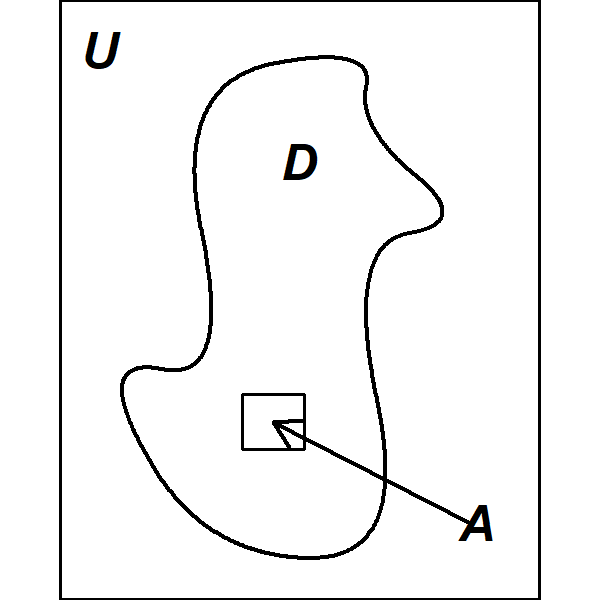
\includegraphics{figure/monteCarlo-region-diagram-1} \end{center}

\begin{center}\rule{0.5\linewidth}{\linethickness}\end{center}

\begin{center}\rule{0.5\linewidth}{\linethickness}\end{center}

\paragraph{The rejection method for dominated
densities}\label{the-rejection-method-for-dominated-densities}

\begin{itemize}
\item
  A useful little fact allows us to extend the rejection method from
  uniform distributions to arbitrary densities.
\item
  @robert04 refer to this fact the \emph{fundamental theorem of
  simulation}.
\end{itemize}

\begin{center}\rule{0.5\linewidth}{\linethickness}\end{center}

\begin{itemize}
\item
  Let \(h\) be an arbitary positive, integrable function.
\item
  Define \[D=\{(x,u): 0{\le}u{\le}h(x)\},\] i.e., \(D\) is the graph of
  \(h\).
\item
  Consider the random pair \((X,U)\!\sim\!\mathrm{uniform}(D)\).
\item
  What is the marginal distribution of \(X\)?
  \[\int_0^{h(x)}\!\mathrm{d}u = h(x)\]
\item
  So \(h\) is the probability distribution function for \(X\)!
\item
  To carry out the rejection method, simulating from \(g\) to obtain a
  sample from \(f\), we take our region \(D\) to be the \textbf{graph}
  of \(Mg\), i.e., \[ D = \{(x,y): 0\le y\le Mg(x),\] where \(M\) is a
  constant chosen so that \(Mg(x)\le f(x)\) for all \(x\).
\item
  We propose points \((X,Y)\) by drawing them uniformly from the area
  under the graph of \(M\,g\).
\item
  We \textbf{accept} the point \((X,Y)\) if it lies under the graph of
  \(f\).
\item
  Then, the \(X\)-component of the \((X,Y)\) pair is distributed
  according to \(f\).
\end{itemize}

\begin{center}\rule{0.5\linewidth}{\linethickness}\end{center}

\begin{itemize}
\item
  This suggests the following rejection method for simulating an
  arbitrary random variable.
\item
  Let \(f\) be the target distribution and \(g\) be another distribution
  function (from which it is easy to simulate) (see Figure below).
\item
  Let \(M\) be such that \(M\,g(x){\ge}f(x)\) for all \(x\).
\item
  The following procedure simulates \(X\!\sim\!f\).
\end{itemize}

\begin{enumerate}
\def\labelenumi{\arabic{enumi}.}
\item
  draw \(Y\!\sim\!g\) and \(U\!\sim\!\mathrm{uniform}(0,M\,g(Y))\).
\item
  if \(U{\le}f(Y)\), then let \(X=Y\) else repeat step 1.
\end{enumerate}

\begin{center}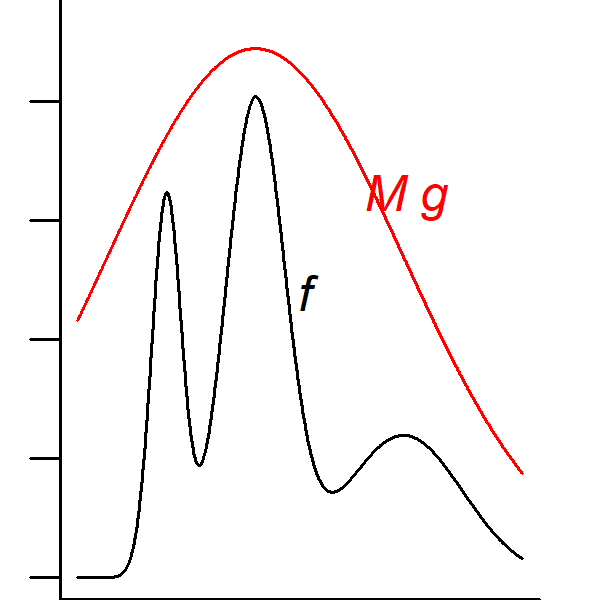
\includegraphics{figure/monteCarlo-rejection-method-diagram-1} \end{center}

\begin{center}\rule{0.5\linewidth}{\linethickness}\end{center}

\begin{center}\rule{0.5\linewidth}{\linethickness}\end{center}

\paragraph{\texorpdfstring{Acknowledgement: These notes derive from
\href{http://kingaa.github.io/sbied/pfilter/monteCarlo.html}{notes by
Aaron
King}.}{Acknowledgement: These notes derive from notes by Aaron King.}}\label{acknowledgement-these-notes-derive-from-notes-by-aaron-king.}


\end{document}
